%template1.tex
%The following LaTeX source file represents the simplest kind of slide presentation; no overlays, no included graphics. Substitute your favorite style for ``pascal''. To create the PDF file template1.pdf, (1) be sure to use the prosper class, then (2) execute the command latex template1.tex, and (3) the command dvipdf template1.dvi.

%%%%%%%%%%%%%%%%%%%%%%%%%%%%%%% template1.tex %%%%%%%%%%%%%%%%%%%%%%%%%%%%%%%%%%%
\documentclass[a4paper,blends,pdf,colorBG,slideColor]{prosper}
% definitions for slides for CSC544
% Lutz Hamel, (c) 2007

\hypersetup{pdfpagemode=FullScreen}

\usepackage{times}
\usepackage{latexsym}
\usepackage{alltt}
\usepackage{booktabs}
\usepackage{amsmath}
\usepackage{amsopn}
\usepackage{amsfonts}
\usepackage{amssymb}
%\usepackage[usenames]{color}

\def\sign{\qopname\relax{no}{sign}}
\def\argmax{\qopname\relax{no}{argmax}}
\def\argmin{\qopname\relax{no}{argmin}}

\newcommand{\grad}{\ensuremath{\nabla}} 
\newcommand{\loss}{\ensuremath{{\cal L}}}
\newcommand{\err}{\mbox{err}}
\newcommand{\mse}{\mbox{mse}}
\newcommand{\acc}{\mbox{acc}}
\newcommand{\Integer}{\ensuremath{\mathbb{N}}}
\newcommand{\size}[1]{{|{#1}|}}
\newcommand{\Rnspace}[1]{\ensuremath{\mathbb{R}^{#1}}}
\newcommand{\Real}{\ensuremath{\mathbb{R}}}
\newcommand{\mytt}[1]{{\small\tt{#1}}}
\newcommand{\textemph}[1]{{\em #1}}
\newcommand{\suchthat}{\mid}
\newcommand{\orbar}{\;|\;}
\newcommand{\bs}[1]{\begin{slide}{#1}\ptsize{8}}
\newcommand{\es}{\end{slide}}
\newcommand{\co}{\,\colon\;}
\newcommand{\pair}[2]{\ensuremath{( {#1}, {#2} )}}
\newcommand{\model}[1]{\hat{#1}}
\newcommand{\ul}[1]{{\bf\em #1}}
\newcommand{\ol}{\overline}
\newcommand{\definition}[1]{{\bf Definition: }{\em #1}}
\newcommand{\example}[1]{{\bf Example: }{#1}}
\newcommand{\abs}[1]{|{#1}|}
\newcommand{\mytab}{\makebox[.1in]{}}

\newcommand{\fdef}[1]{
\begin{center}
\fbox{
\begin{minipage}{3.5in}
{\bf Definition:}
{#1}
\end{minipage}
}
\end{center}
}

\newcommand{\fframe}[1]{
\begin{center}
\fbox{
\begin{minipage}{3.5in}
{#1}
\end{minipage}
}
\end{center}
}

\newcommand{\nframe}[1]{
\begin{center}
\begin{minipage}{3.5in}
{#1}
\end{minipage}
\end{center}
}

\newenvironment{Rcode}
	{
		\scriptsize
		\begin{quote}
		\begin{alltt}
	}
	{
		\end{alltt}
		\end{quote}
	}




\begin{document}

\bs{One-versus-the-Rest}

We extend SVM's in order to support multi-class classification problems.

Consider the training dataset
\[
D = \{(\ol{x}_1,y_1), (\ol{x}_2,y_2),\ldots,(\ol{x}_l,y_l)\} \subset \Rnspace{n} \times \{1,\ldots,M\},
\]
where the label $y_i$ can take on any label in $\{1,\ldots,M\}$ with $i = 1,\ldots,n$ and $M > 2$.

The most popular technique for multi-class classification 
is called \ul{one-versus-the-rest} classification.  

Here we build $M$ decision surfaces, say $g^1,\ldots,g^M$, each trained to separate one
class from the rest.
That is, the decision surface $g^1$ is trained to separate the class labeled $1$ from all other classes,
the decision surface $g^2$ is trained to separate the class labeled $2$ from all other classes, {\it etc.}

In order to classify an unknown point $\ol{x}$ we use a \ul{voting scheme} based
on which one of the $M$ decision surfaces returns the \ul{largest value} for the point $\ol{x}$.
We interpret this as selecting the decision surface that separates the point $\ol{x}$ with the \ul{highest confidence} from the
majority of points.

\es

\bs{Models: Training Sets}
In order to train $M$ binary
decision surfaces we have to construct appropriate binary training datasets.

Let $p \in \{1,\ldots,M\}$, then for each decision surface $g^p$ we construct the binary training set
$D^p = D_{+}^p \cup D_{-}^p$ where

\begin{eqnarray*}
D_{+}^p &=& \{(\ol{x},+1) \mid (\ol{x},y) \in D \wedge y = k \},\\
D_{-}^p &=& \{(\ol{x},-1) \mid (\ol{x},y) \in D \wedge y \neq k \}.
\end{eqnarray*}

{\bf Observation:} The set $D_{+}^p$ contains all the points that are members of the class $p$ and
the set $D_{-}^p$ contains all the remaining points.
\es

\bs{Models: Decision Surfaces}
Using our binary training datasets we construct the decision surfaces
\[
g^p(\ol{x}) = \sum_{i=1}^{\abs{D^p}} y_i^p\alpha_i^p k(\ol{x}_i,\ol{x}) - b^p
\]
with $p \in \{1,\ldots,M\}$ and $(\ol{x}_i,y_i)\in D^p$.

\vspace{.2in}
{\bf Note:} The function $g^p(\ol{x})$ returns a signed real value and this value
can be interpreted as the distance from the decision surface to the point $\ol{x}$.
This value can also be interpreted as a \ul{confidence value}; the larger the value
the more confident we are that the point $\ol{x}$ belong to the positive class.

\es

\bs{Models: Voting Scheme}
We can use the confidence value as our criterion to pick the best decision surface: we pick the
decision surface with the largest confidence value.  That is, we assign point $\ol{x}$
to the class whose decision surface returns the largest value for this point.  

More formally, we can construct the decision function $\model{f}\co \Rnspace{n} \rightarrow \{1,\ldots,M\}$ 
for our multi-class
classification problem as follows,
\fframe{
\[
\model{f}(\ol{x}) = \argmax_k g^p(\ol{x}),
\]}
where $p \in \{1,\ldots,M\}$ and $\ol{x}\in \Rnspace{n}$.  

{\bf Note:}The function $\argmax$ returns the value of $p$ that 
maximizes the function $g^p$.

\es

\bs{An Example}
As an example we look at a classification problem with three classes where
the training dataset $D$ is defined as
\begin{equation*}
D = \{(\ol{x}_1,y_1), (\ol{x}_2,y_2),\ldots,(\ol{x}_l,y_l)\} \subset \Rnspace{2} \times \{1,2,3\},
\end{equation*}
with $l = 9$.

\begin{center}
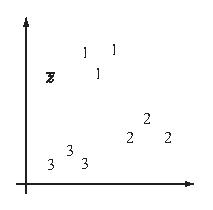
\includegraphics[height=40mm]{figures/fig11-01.eps}
\end{center}
The label of point $\ol{z}$ is unknown and should be estimated from the dataset.
\es

\bs{An Example}
{\small
We can proceed with our construction and build three training datasets, one
for each decision surface that separates one class from the rest,
\begin{eqnarray}
D^1 &=& D_{+}^1 \cup D_{-}^1, \nonumber \\
D^2 &=& D_{+}^2 \cup D_{-}^2, \nonumber \\
D^3 &=& D_{+}^3 \cup D_{-}^3. \nonumber
\end{eqnarray}
We then construct the decision surfaces, $g^1$, $g^2$, and $g^3$, one for each of 
these datasets, respectively.
\begin{center}
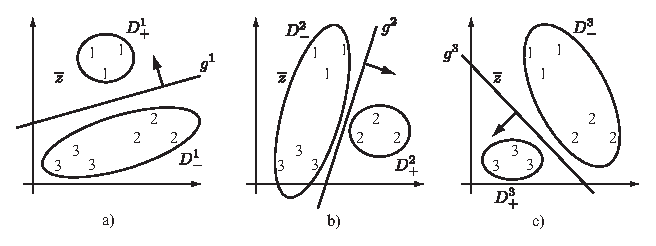
\includegraphics[height=35mm]{figures/fig11-02.eps}
\end{center}
Now: for $\model{f}\co \Rnspace{n} \rightarrow \{1,2,3\}$, $\model{f}(\ol{z}) = ?$
}
\es

\bs{An Example}
\vspace{.2in}
{\bf Observation:} The training sets for the individual decision surfaces in one-versus-the-rest tend to be highly unbalanced.

\es


\bs{Pairwise Classification}
\small
Solution: build decision surfaces for \ul{each pair of classes}.

Given the training  set 
\begin{equation*}
D = \{(\ol{x}_1,y_1), (\ol{x}_2,y_2),\ldots,(\ol{x}_l,y_l)\} \subset \Rnspace{n} \times \{1,2,\ldots,M\},
\end{equation*}
we let $g^{p,q}\co \Rnspace{n} \rightarrow \{p,q\}$ denote the decision surface
that separates the pair of classes $p$ and $q$  with $p \ne q$ and $\{p,q\} \subset \{1,2,\ldots,M\}$.
We train each decision surface,
\begin{equation*}
g^{p,q}(\ol{x}) = \sum_{i=1}^{\size{D^{p,q}}} y_i\alpha_i^{p,q} k(\ol{x}_i,\ol{x}) - b^{p,q},
\end{equation*}
on the data set,
\begin{equation*}
D^{p,q} = D^p \cup D^q,
\end{equation*}
where
\begin{align*}
D^p &= \{ (\ol{x},y) \suchthat  (\ol{x},y) \in D \wedge y = p\},\\
\intertext{and}
D^q &= \{ (\ol{x},y) \suchthat  (\ol{x},y) \in D \wedge y = q\}.
\end{align*}
\es

\bs{Pairwise Classification}

\vspace{.2in}

Once we have constructed all the pairwise decision surfaces $g^{p,q}$ using the
corresponding training sets $D^{p,q}$, we can classify an unknown
point by applying each of the $M(M-1)/2$ decision surfaces to
this point keeping track of how many times the point was assigned to what class label.
The class label with the highest count is then considered the label for the unknown point.

\es

\bs{Pairwise Classification}
\scriptsize
\fframe{
{\rm\it // multi-class training set }\\
{\bf let} $D = \{(\ol{x}_1,y_1), (\ol{x}_2,y_2),\dots,(\ol{x}_l,y_l)\} \subset \Rnspace{n} \times \{1,2,\ldots,M\}$\\
{\rm\it // point to be classified}\\
{\bf let} $\ol{z}\in\Rnspace{n}$\\
{\rm\it // initialize the counter for the labels to zero}\\
{\bf let} $cnt[1\ldots M] = \ol{0}$\\
{\rm\it // loop through all possible pairs of labels}\\
{\bf for} $p = 1$ {\bf to} $M$ {\bf do}\\
\mytab{\bf for} $q = p+1$ {\bf to} $M$ {\bf do}\\
\mytab\mytab {\rm\it // construct the decision surface for this pair of labels}\\
\mytab\mytab {\bf let} $D^{p,q} = D^p \cup D^q$\\
\mytab\mytab {\bf train} $g^{p,q}$ {\bf on} $D^{p,q}$\\
\mytab\mytab {\rm\it // classify the unknown point with the current decision surface}\\
\mytab\mytab {\rm\it // and increment the appropriate counter}\\
\mytab\mytab {\bf if} $g^{p,q}(\ol{z}) == p$ {\bf then}\\
\mytab\mytab\mytab $cnt[p]++$\\
\mytab\mytab{\bf else}\\
\mytab\mytab\mytab $cnt[q]++$\\
\mytab\mytab{\bf end if}\\
\mytab {\bf end for}\\
{\bf end for}\\
{\rm\it // return the label with the largest count}\\
{\bf return} $\argmax_{i = 1,\ldots, M} \left (cnt[i] \right )$
}
\es

\bs{An Example}
Consider the same training set from before,
\begin{equation*}
D = \{(\ol{x}_1,y_1), (\ol{x}_2,y_2),\ldots,(\ol{x}_l,y_l)\} \subset \Rnspace{2} \times \{1,2,3\},
\end{equation*}
with $l = 9$.

\begin{center}
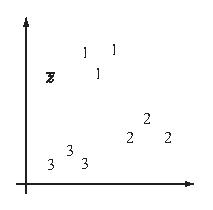
\includegraphics[height=40mm]{figures/fig11-01.eps}
\end{center}
The label of point $\ol{z}$ is unknown and should be estimated from the dataset.
\es

\bs{An Example}
\begin{center}
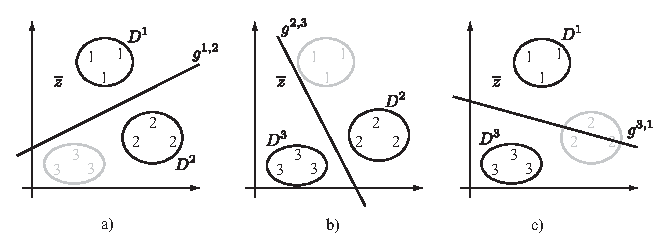
\includegraphics[height=40mm]{figures/fig11-03.eps}
\end{center}
The three training data sets, $D^{p}\cup D^q$ 
and the corresponding decision surfaces $g^{p,q}$ with $\{p,q\} \subset \{1,2,3\}$;
part a) shows the case for $p=1$ and $q=2$, part b) 
for $p=2$ and $q=3$, and part c) for $p=3$ and $q=1$.   Here, the point $\ol{z}$ belongs to class $1$ because the largest score,
\begin{center}
   \begin{tabular}{ccc}
     % \toprule
  Class $1$ & Class $2$ & Class $3$ \\
     \midrule
      $2$     & $0$ & $1$ \\ 
      %\bottomrule
   \end{tabular}
\end{center}

\es

\bs{Observations}
\begin{itemize}
\item
Both the One-versus-the-Rest and the Pairwise Classification schemes coincide in the classification
of point $\ol{z}$.

\item
In pairwise classification the training sets are more balanced, however, we have to construct $M(M-1)/2$
of them together with their corresponding decision surfaces.

\item 
The package 'e1071' implements the pairwise classification scheme for multi-class classification.
\end{itemize}
\es


\end{document}
%%%%%%%%%%%%%%%%%%%%%%%%%%% end of template1.tex %%%%%%%%%%%%%%%%%%%%%%%%%%%%%%%%

